% !TEX encoding = UTF-8
% !TEX TS-program = pdflatex
% !TEX root = ../tesi.tex
% !TEX spellcheck = it-IT

%**************************************************************
\chapter{Il progetto di stage}
\label{cap:progetto-stage}

%**************************************************************
\section{Il contesto}
\label{sec:contesto}
La piattaforma Plot è composta da due moduli Laravel distinti: un modulo di gioco ed un modulo CMS.
\\ \\
Il \textbf{modulo di gioco} incorpora la logica necessaria all'utente per interagire con la piattaforma. Questo modulo permette quindi agli utenti finali di:
\begin{itemize}
	\item Autenticarsi;
	\item Invitare altri utenti a far parte della propria squadra;
	\item Accedere al contenuto delle mission;
	\item Accedere al contenuto dei post;
	\item Accedere e rispondere alle question che vengono loro proposte;
	\item Accedere alle informazioni riguardanti il proprio team;
	\item Consultare la classifica generale.
\end{itemize}

Il \textbf{modulo CMS} incorpora la logica necessaria agli amministratori per gestire il Plot. Questo modulo permette quindi agli amministratori di:
\begin{itemize}
	\item Autenticarsi;
	\item Creare nuove mission;
	\item Eliminare mission esistenti;
	\item Modificare i dettagli di una particolare mission;
	\item Accedere all'elenco di tutte le mission;
	\item Creare nuovi post per una particolare mission;
	\item Eliminare post esistenti;
	\item Modificare i dettagli di un particolare post;
	\item Accedere all'elenco di tutti i post relativi ad una particolare mission;
	\item Creare nuove question per un particolare post;
	\item Eliminare question esistenti;
	\item Modificare i dettagli di una particolare question;
	\item Accedere all'elenco di tutte le question relative ad un particolare post;
	\item Accedere all'elenco degli utenti iscritti alla piattaforma;
	\item Eliminare utenti esistenti;
	\item Modificare i dettagli di un particolare utente;
	\item Accedere all'elenco dei compagni di team di un particolare utente;
	\item Accedere all'elenco dei team;
	\item Eliminare team esistenti;
	\item Modificare i dettagli di un particolare team;
	\item Accedere all'elenco dei componenti di un particolare team;
	\item Accedere alla classifica generale;
	\item Accedere all'elenco delle domande previste, corredate delle risposte corrette  e del tipo di post al quale sono associate;
	\item Accedere all'elenco delle risposte fornite dagli utenti.
\end{itemize}

Entrambi i moduli Laravel utilizzano il medesimo database MySQL per la persistenza dei dati (Figura~\ref{fig:coupled}). 
Il database, pensato inizialmente per Vodafone, è stato adattato per diversi Plot, modificandolo di volta in volta. Le continue modifiche hanno portato ad avere un database inconsistente e poco manutenibile, a causa anche della scarsa documentazione.
\\ \\
Ogni modulo Laravel prevede un front end collegato ad un relativo back end. Le logiche che sottendono i due back end sono, però, molto simili e questo porta ad avere codice duplicato e poco manutenibile.
\\ \\
Ulteriori problematiche nascono dal fatto che entrambi i front end sono fortemente accoppiati al relativo back end, questo implica una struttura poco modulare e difficilmente riusabile.
\\ \\
Nel prosieguo della trattazione, con l’appellativo “Plot 1.0” mi riferirò alla configurazione della piattaforma esistente prima dell'inizio del progetto di stage.

\begin{figure}[htbp]
\begin{center}
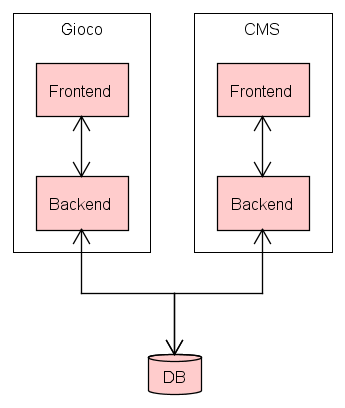
\includegraphics[height=8cm]{coupled-diagram}
\caption{Organizzazione della piattaforma prima del progetto di stage}
\label{fig:coupled}
\end{center}
\end{figure}

%**************************************************************
\section{Descrizione del progetto}
Il progetto di stage prevede tre attività principali:
\begin{enumerate}
	\item Refactoring del database che consente la persistenza dei dati utili alla piattaforma Plot;
	\item Creazione di un set di API REST che permettano di interagire con il database (di cui al punto 1);
	\item Refactoring del front end relativo al CMS.
\end{enumerate}

La piattaforma Plot è in continua evoluzione e mira ad adattarsi, quanto più possibile, alle richieste dei clienti. Le attività di progetto devono quindi essere affrontate con l'obiettivo di massimizzare la modularizzazione, in modo da consentire una buona manutenibilità della piattaforma ed un basso accoppiamento tra le parti.
\\ \\
Dato il respiro internazionale e multinazionale dei potenziali clienti della piattaforma, deve essere implementato il concetto di \textbf{traducibilità}: ogni risorsa di testo importante ai fini del gioco deve poter essere localizzata in base alla lingua preferita dall'utente che ne usufruisce.
\\ \\
Mantenere uno storico delle azioni effettuate dai giocatori può risultare utile per individuare la causa di eventuali problemi inaspettati, si richiede quindi di prevedere un meccanismo di \textbf{logging} che registri e renda accessibili le richieste HTTP effettuate dai giocatori.
\\ \\
Il set di API REST ed il front end del CMS dovranno consentire di effettuare tutte le operazioni già disponibili dall'interfaccia grafica del CMS di Plot 1.0 (elencate nella sezione "`\hyperref[sec:hello]{Il contesto}"`). 
In aggiunta alle operazioni già note, dovrà essere possibile:
\begin{itemize}
	\item Accedere all'elenco degli amministratori della piattaforma;
	\item Eliminare gli amministratori;
	\item Modificare i dettagli di un particolare amministratore;
	\item Accedere all'elenco dei log generati dagli utenti del front end di gioco;
	\item Accedere all'elenco delle traduzioni disponibili per una data risorsa;
	\item Eliminare le traduzioni relative ad una data risorsa;
	\item Modificare i dettagli di un particolare traduzione.
\end{itemize}

Non è richiesta un'interfaccia grafica professionale per il modulo CMS.

%**************************************************************
\section{Tecnologie utilizzate}
\subsection{Database}
Per gestire il database è stato scelto \textbf{MySQL Workbench}: uno strumento di amministrazione visuale che permette di creare e modificare agevolmente lo schema di un database MySQL.
\\ \\
La scelta è ricaduta su questo strumento in quanto: 
\begin{itemize}
	\item Ufficialmente supportato e consigliato dalla comunità MySQL;
	\item Fornisce un procedimento assistito per la creazione dello schema, facilitando l'individuazione di errori.
\end{itemize}

\begin{figure}[htbp]
\begin{center}

\includegraphics[height=2cm]{logos/mysql-workbench-logo}
\caption{Logo MySQL Workbench}
\end{center}
\end{figure}

\subsection{Framework}
\subsubsection{Back end}
Il framework principale utilizzato per il progetto è \textbf{Laravel}: un framework PHP open-source, pensato per la creazione di applicazioni web basate sul pattern architetturale MVC (Model-View-Controller). 
\\ \\
Il framework è stato scelto dall'azienda per i vantaggi che offre, tra i quali:
\begin{itemize}
	\item Una documentazione ampia e facilmente consultabile in rete;
	\item Una sintassi pulita ed intuitiva;
	\item Facilità di implementazione della dependency injection;
	\item \textit{Eloquent}: ORM integrato di Laravel;
	\item \textit{Blade}: il template engine integrato di Laravel.
\end{itemize}

\begin{figure}[htbp]
\begin{center}

\includegraphics[height=2cm]{logos/laravel-logo-white}
\caption{Logo Laravel}
\end{center}
\end{figure}

\subsubsection{Front end}
Per il refactoring dell'interfaccia grafica del CMS è stato utilizzato \textbf{Bootstrap}: un framework HTML, CSS e JavaScript per la creazione di pagine web responsive e mobile-first.
\\ \\
Il framework è stato scelto perchè:
\begin{itemize}
	\item Mette a disposizione tutti i componenti base e gli stili utili per la creazione di una pagina web (layout a griglia, tabelle, box modali, form e molto altro);
	\item Viene supportato da tutti i maggiori browser;
	\item Permette di creare interfacce grafiche consistenti, anche senza modificare le componenti fornite;
	\item Pensato per creare pagine responsive che si adattino anche ai dispositivi mobile;
	\item Include un set di icone pronte all'uso;
	\item Ha una buona documentazione ed un grande supporto dalla comunità;
	\item Esistono molti temi, template e plugin gratuiti.
\end{itemize}

Oltre ai molti pregi, questo framework porta con sé almeno due difetti: 
\begin{itemize}
	\item Produce codice HTML verboso che può risultare non perfettamente semantico;;
	\item Molti componenti non funzionano se JavaScript è disattivato.
\end{itemize}

In accordo con l'azienda, questi non sono stati ritenuti problemi bloccanti in quanto il CMS verrà ospitato su un server privato e sarà ad uso esclusivo degli amministratori, che avranno cura di utilizzare un browser che supporti JavaScript.

\begin{figure}[htbp]
\begin{center}

\includegraphics[height=2cm]{logos/bootstrap-logo}
\caption{Logo Bootstrap}
\end{center}
\end{figure}

\subsection{Versionamento}
Per il versionamento del codice è stato è stato utilizzato \textbf{Bitbucket} con base \textbf{Git}, in quanto già in uso presso l'azienda.
Bitbucket è un servizio di web-hosting per progetti software che utilizzano Git o Mercurial come sistemi di versionamento.
\\ \\
Il punto di forza di Bitbucket è la possibilità di creare, gratuitamente, repository privati. Questo risulta fondamentale per un'azienda che voglia mantenere il codice dei propri progetti accessibile solo a determinate persone.

\begin{figure}[htbp]
\begin{center}

\includegraphics[height=2cm]{logos/Atlassian_Bitbucket_Logo}
\caption{Logo Bitbucket}
\end{center}
\end{figure}

Git è un software per il versionamento distribuito ed è stato scelto dall'azienda in quanto offre:
\begin{itemize}
	\item Semplicità di utilizzo;
	\item Una buona documentazione disponibile online;
	\item La possibilità di lavorare anche offline, in quanto ogni sviluppatore possiede una copia locale del repository sul quale può effettuare commit anche in assenza di connessione. 
\end{itemize} 

\begin{figure}[htbp]
\begin{center}

\includegraphics[height=1.5cm]{logos/git-logo}
\caption{Logo Git}
\end{center}
\end{figure}

\subsection{Gestione di progetto}
Per la gestione di progetto è stato è stato utilizzato \textbf{Basecamp}, in quanto già in uso presso l'azienda.
\\ \\
Basecamp è un servizio web per che permette di condividere e organizzare tutto ciò che è necessario per la gestione di un progetto: task, discussioni, deadline e file.

\begin{figure}[htbp]
\begin{center}

\includegraphics[height=1.5cm]{logos/Basecamp-logo}
\caption{Logo Basecamp}
\end{center}
\end{figure}